\documentclass[11pt]{article}
\usepackage[margin=1in]{geometry}          
\usepackage{graphicx}
\usepackage{listings}
\usepackage[T1]{fontenc}
\usepackage[american]{babel}
\usepackage{fancyvrb}
\usepackage{bm}
\usepackage[svgnames]{xcolor}
\usepackage{amsthm, amsmath, amssymb}
\usepackage[loose,nice]{units} %replace "nice" by "ugly" for units in upright fractions
 
\title{Spatio-temporal Data Analysis HW1}
\author{2020311198 Dongook Son}
\date{Spring 2020}

\lstset{% setup listings
  language=R,% set programming language
  basicstyle=\ttfamily\small,% basic font style
  backgroundcolor=\color{WhiteSmoke},
  keywordstyle=\color{blue},% keyword style
  commentstyle=\color{gray},% comment style
  numbers=left,% display line numbers on the left side
  numberstyle=\scriptsize,% use small line numbers
  numbersep=10pt,% space between line numbers and code
  tabsize=3,% sizes of tabs
  showstringspaces=false,% do not replace spaces in strings by a certain character
  captionpos=b,% positioning of the caption below
  breaklines=true,% automatic line breaking
  escapeinside={(*}{*)},% escaping to LaTeX
  fancyvrb=true,% verbatim code is typset by listings
  extendedchars=false,% prohibit extended chars (chars of codes 128--255)
  literate={"}{{\texttt{"}}}1{<-}{{$\bm\leftarrow$}}1{<<-}{{$\bm\twoheadleftarrow$}}1
  {~}{{$\bm\sim$}}1{<=}{{$\bm\le$}}1{>=}{{$\bm\ge$}}1{!=}{{$\bm\neq$}}1{^}{{$^{\bm\wedge}$}}1,% item to replace, text, length of chars
  alsoletter={.<-},% becomes a letter
  alsoother={$},% becomes other
  otherkeywords={!=, ~, $, \&, \%/\%, \%*\%, \%\%, <-, <<-, /},% other keywords
  deletekeywords={c}% remove keywords
}

\begin{document}
\maketitle

\section*{Q1}
\subsection*{(a)}
Prove $E(Y)=E(\mu+LZ)$ and $V(Y)=V(\mu+LZ)$

\begin{proof}
  \begin{align*}
    E(Y) &= E(\mu + LZ) \\
    &= \mu+E(LZ) \\
    &= \mu+LE(Z) & \text{(linearity property)} \\
    &= \mu \\
    V(Y) &= E([(Y-E(Y))(Y-E(Y))']) \\
    &= E([(Y-\mu)(Y-\mu)']) \\
    &= E([(LZ)(LZ)']) \\
    &= E([LZZ'L']) \\
    &= LE(ZZ')L' \\
    &= LV(Z)L' \\
    &= LIL' \\
    &= LL' \\
    &= \Sigma
  \end{align*}
\end{proof}

\subsection*{(b)}

\begin{lstlisting}
  create_multivariate_normal <- function (mu, Sigma) {
  lower_triangle_matrix <- t(chol(Sigma))
  dimension <- nrow(Sigma)
  Z <- rmvnorm(n = 1, mean = rep(0, dimension), sigma = diag(dimension))
  Y = mu + lower_triangle_matrix %*% Z
  return(Y)
}
\end{lstlisting}
\subsection*{(c)}
 \begin{lstlisting}
library(mvtnorm)
library(clusterGeneration)
library(yarrr)
generate_z <- function(dimension, seed= 1) {
  set.seed(seed)
  Z <- rmvnorm(n = 1, mean = rep(0, dimension), sigma = diag(dimension))
  return(Z)
}

generate_multivariate_normal_with_Z <- function (mu, Sigma, Z, seed=1) {
  set.seed(seed)
  lower_triangle_matrix <- t(chol(Sigma))
  Y = mu + (lower_triangle_matrix %*% t(Z))
  return(Y)
}


dimension <- 100
Z_sample <- generate_z(dimension)

plot(x=1,
     type="n",
     xlim = c(1,100),
     ylim = c(-10,10),
     pch = 16,
     xlab="Sample Index",
     ylab="Y_sample",
     )
grid()

set.seed(1)
Sigma <- genPositiveDefMat(dimension, covMethod="eigen")$Sigma
Y_sample <- generate_multivariate_normal_with_Z(mu = rep(0,100), Sigma = Sigma, Z = Z_sample)
points(1:100, Y_sample,
       pch = 16,
       col = transparent("coral2", trans.val = .8))

set.seed(1)
Sigma <- genPositiveDefMat(dimension, covMethod="onion")$Sigma
Y_sample <- generate_multivariate_normal_with_Z(mu = rep(0,100), Sigma = Sigma, Z = Z_sample)
points(1:100, Y_sample,
       pch = 16,
       col = transparent("coral", trans.val = .5))

set.seed(1)
Sigma <- genPositiveDefMat(dimension, covMethod="unifcorrmat")$Sigma
Y_sample <- generate_multivariate_normal_with_Z(mu = rep(0,100), Sigma = Sigma, Z = Z_sample)
points(1:100, Y_sample,
       pch = 16,
       col = transparent("coral3", trans.val = .3))

Sigma <- diag(dimension)
Y_sample <- generate_multivariate_normal_with_Z(mu = rep(0,100), Sigma = Sigma, Z = Z_sample)
points(1:100, Y_sample,
       pch = 12,
       col = transparent("blue", trans.val = .1))
\end{lstlisting}
\begin{figure}[h!]
\center{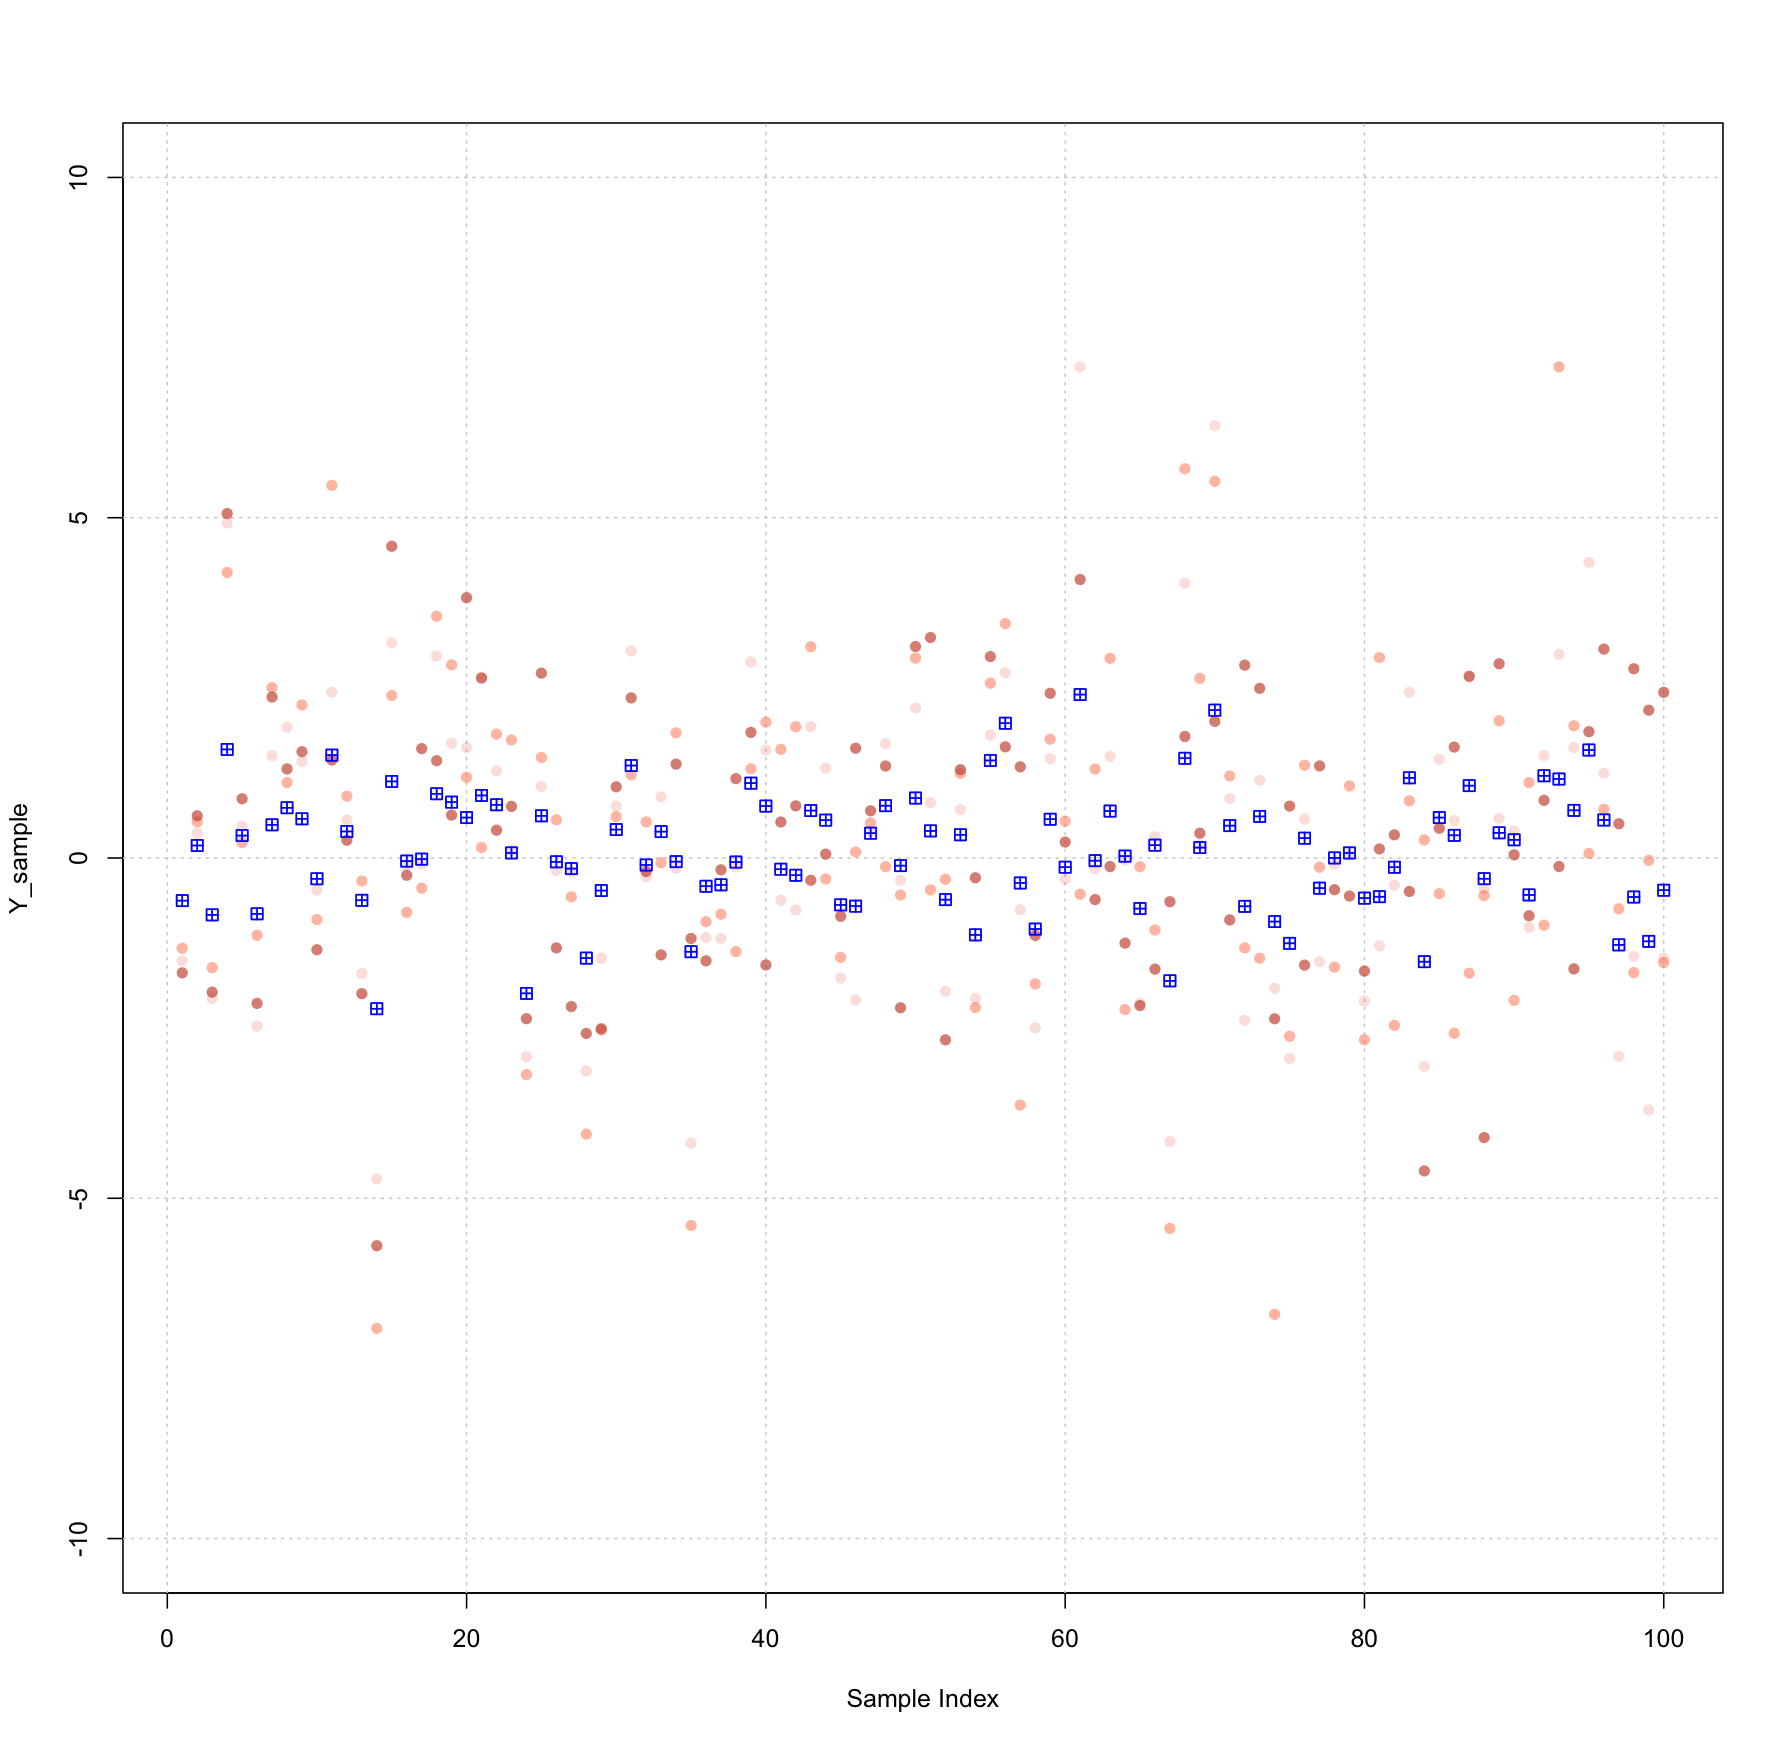
\includegraphics[scale=0.18]{image.png}}
\end{figure}
The blue squares are samples from an identity matrix sigma and others are from correlated sigmas.

\section*{Q2}
\subsection*{(a)}
    \begin{lstlisting}
CAtemp_with_coordinates <- cbind(CAtemp, coordinates(CAtemp))
ordinary_least_squares <- lm(avgtemp ~ lon + lat + elevation, data = CAtemp_with_coordinates)
predictions <- predict(ordinary_least_squares, newdata = CAtemp_with_coordinates)
residuals <- CAtemp_with_coordinates$avgtemp - predictions
CAtemp_with_residuals <- cbind(CAtemp_with_coordinates, residuals); names(CAtemp_with_residuals)[5] <- 'residuals'

range(CAtemp_with_residuals$residuals)
breaks <- -7:7
ploteqc(CAtemp_with_residuals, CAtemp_with_residuals$residuals, breaks, pch = 19)
map("county", region = "california", add = TRUE)
title(main = "Residual plot")
    \end{lstlisting}

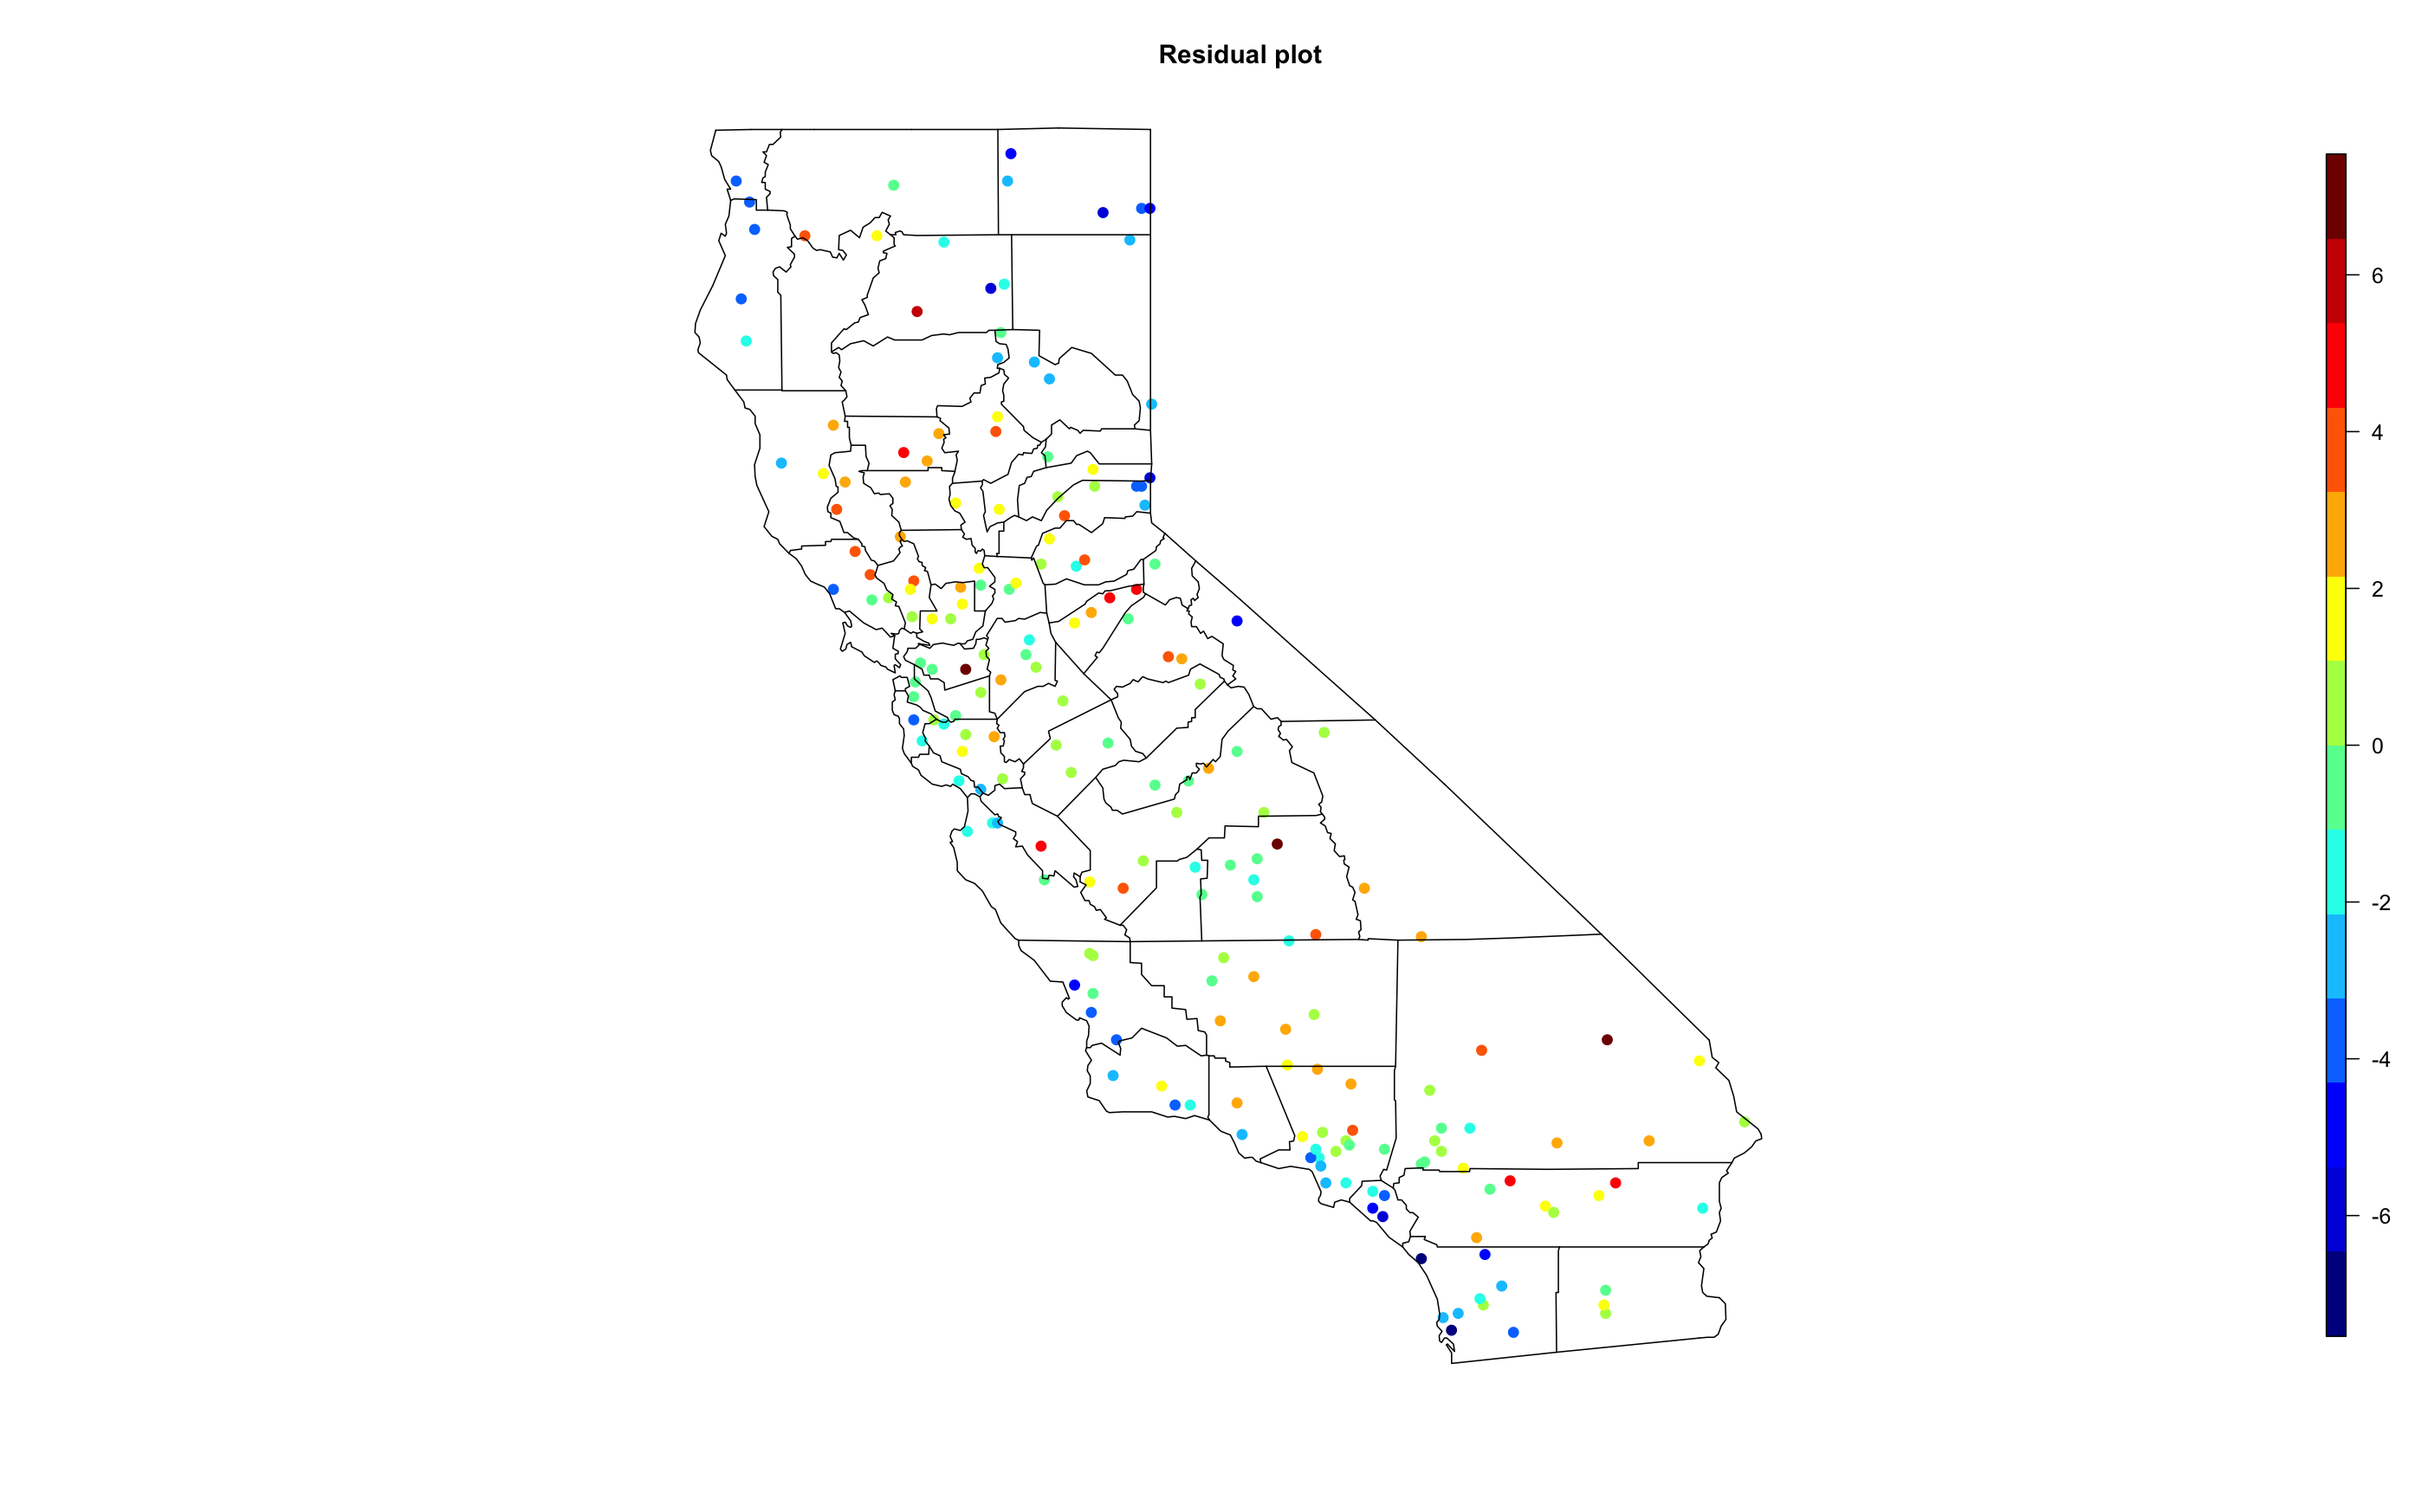
\includegraphics[scale=0.1]{residual_plot.png}

Plot of residuals as colored points onto map of CA. \\
Residuals seem to have a shrinking pattern as it gets closer to the border.
This means that there lies unmeasured spatial dependency for the data.
\begin{lstlisting}
par(mfrow = c(1,2))
range(CAtemp$avgtemp)
breaks <- 40:75
ploteqc(CAtemp, CAtemp$avgtemp, breaks, pch = 19)
map("county", region = "california", add = TRUE)
title(main = "Average Annual Temperatures, 1961-1990, Degrees F")
ploteqc(CAtemp_with_predictions, CAtemp_with_predictions$predictions, breaks, pch = 19)
map("county", region = "california", add = TRUE)
title(main = "Prediction plot")
\end{lstlisting}

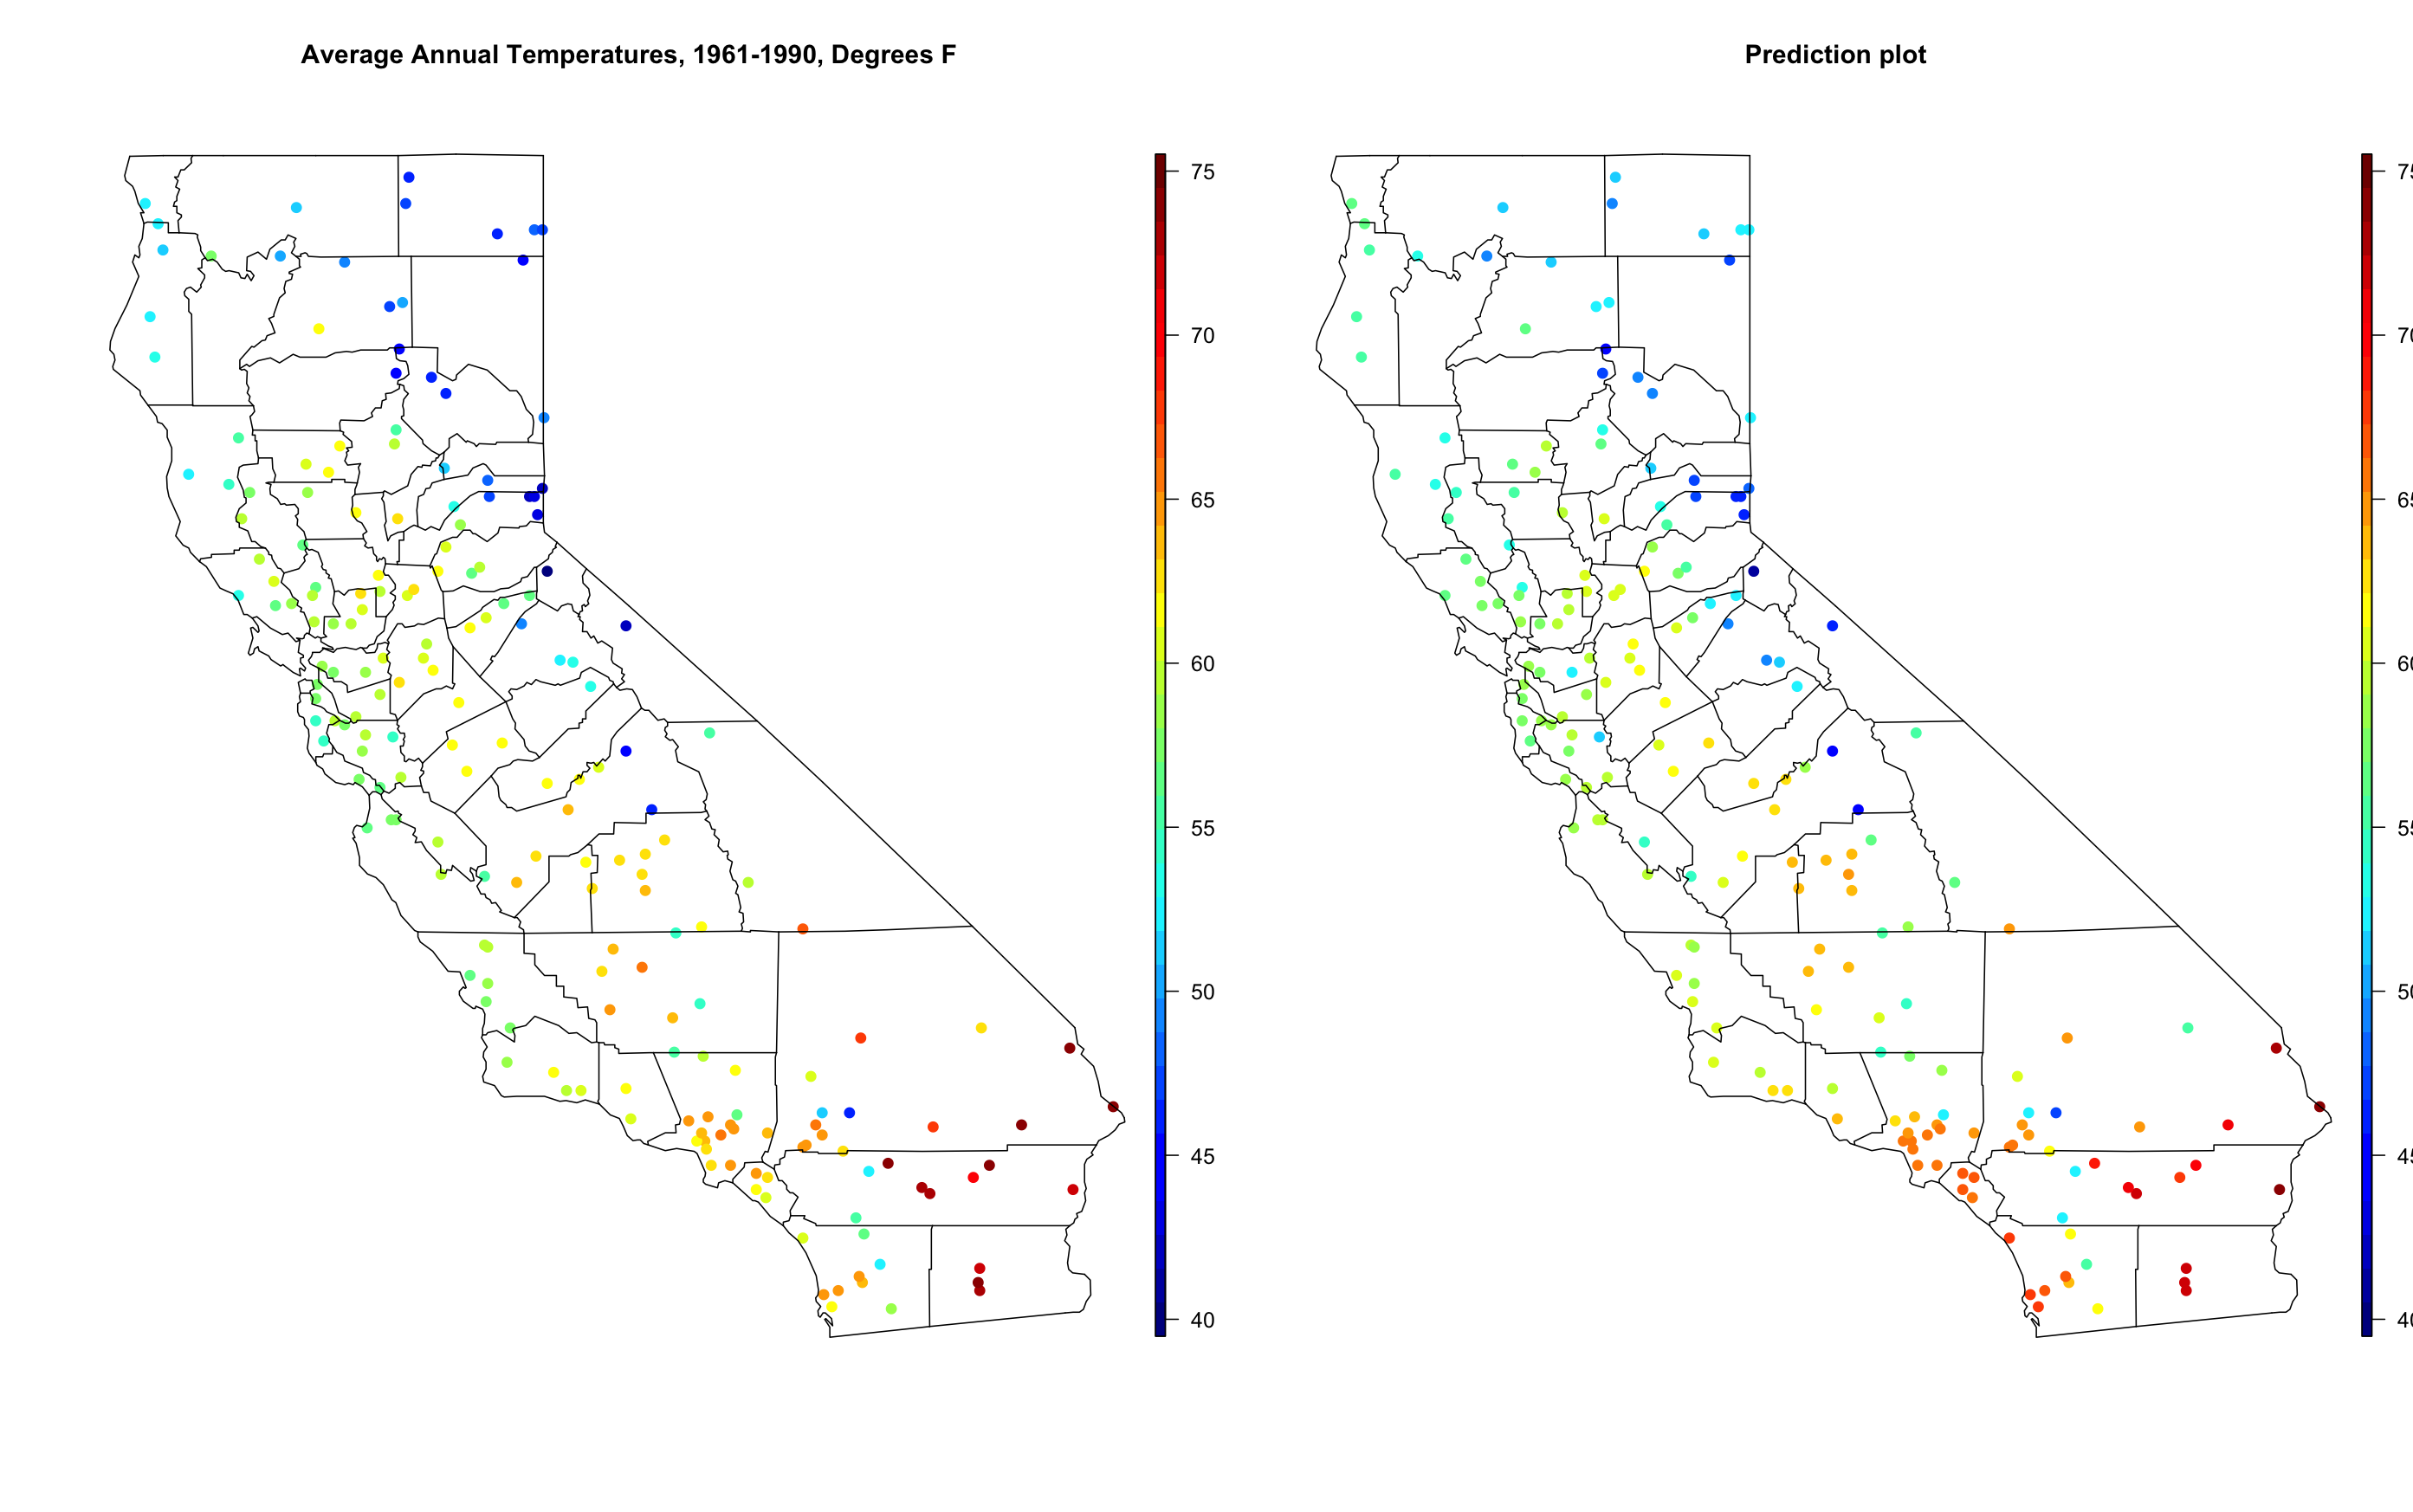
\includegraphics[scale=0.18]{prediction_plot.png}
This is the prediction plot side by side with the original data.

\subsection*{(b)}
After non-parametric variogram estimation we can fit a exponential(parametric) curve using the residuals.
The parameters are as follows. \\
$
\hat{\tau}^2 = 1.978, \hat{\sigma}^2 = 4.804, \hat{\rho}^2 = 88.937.
$
\begin{lstlisting}
variogram <- variogram(residuals ~ 1, data = CAtemp_with_coordinates)
variogram.fit <- fit.variogram(variogram, vgm(1, "Exp", 100, 2))
plot(variogram, variogram.fit)

sigma_sqrd_hat <- variogram.fit$psill[2]
tau_sqrd_hat <- variogram.fit$psill[1]
rho_hat <- variogram.fit$range[2]
\end{lstlisting}

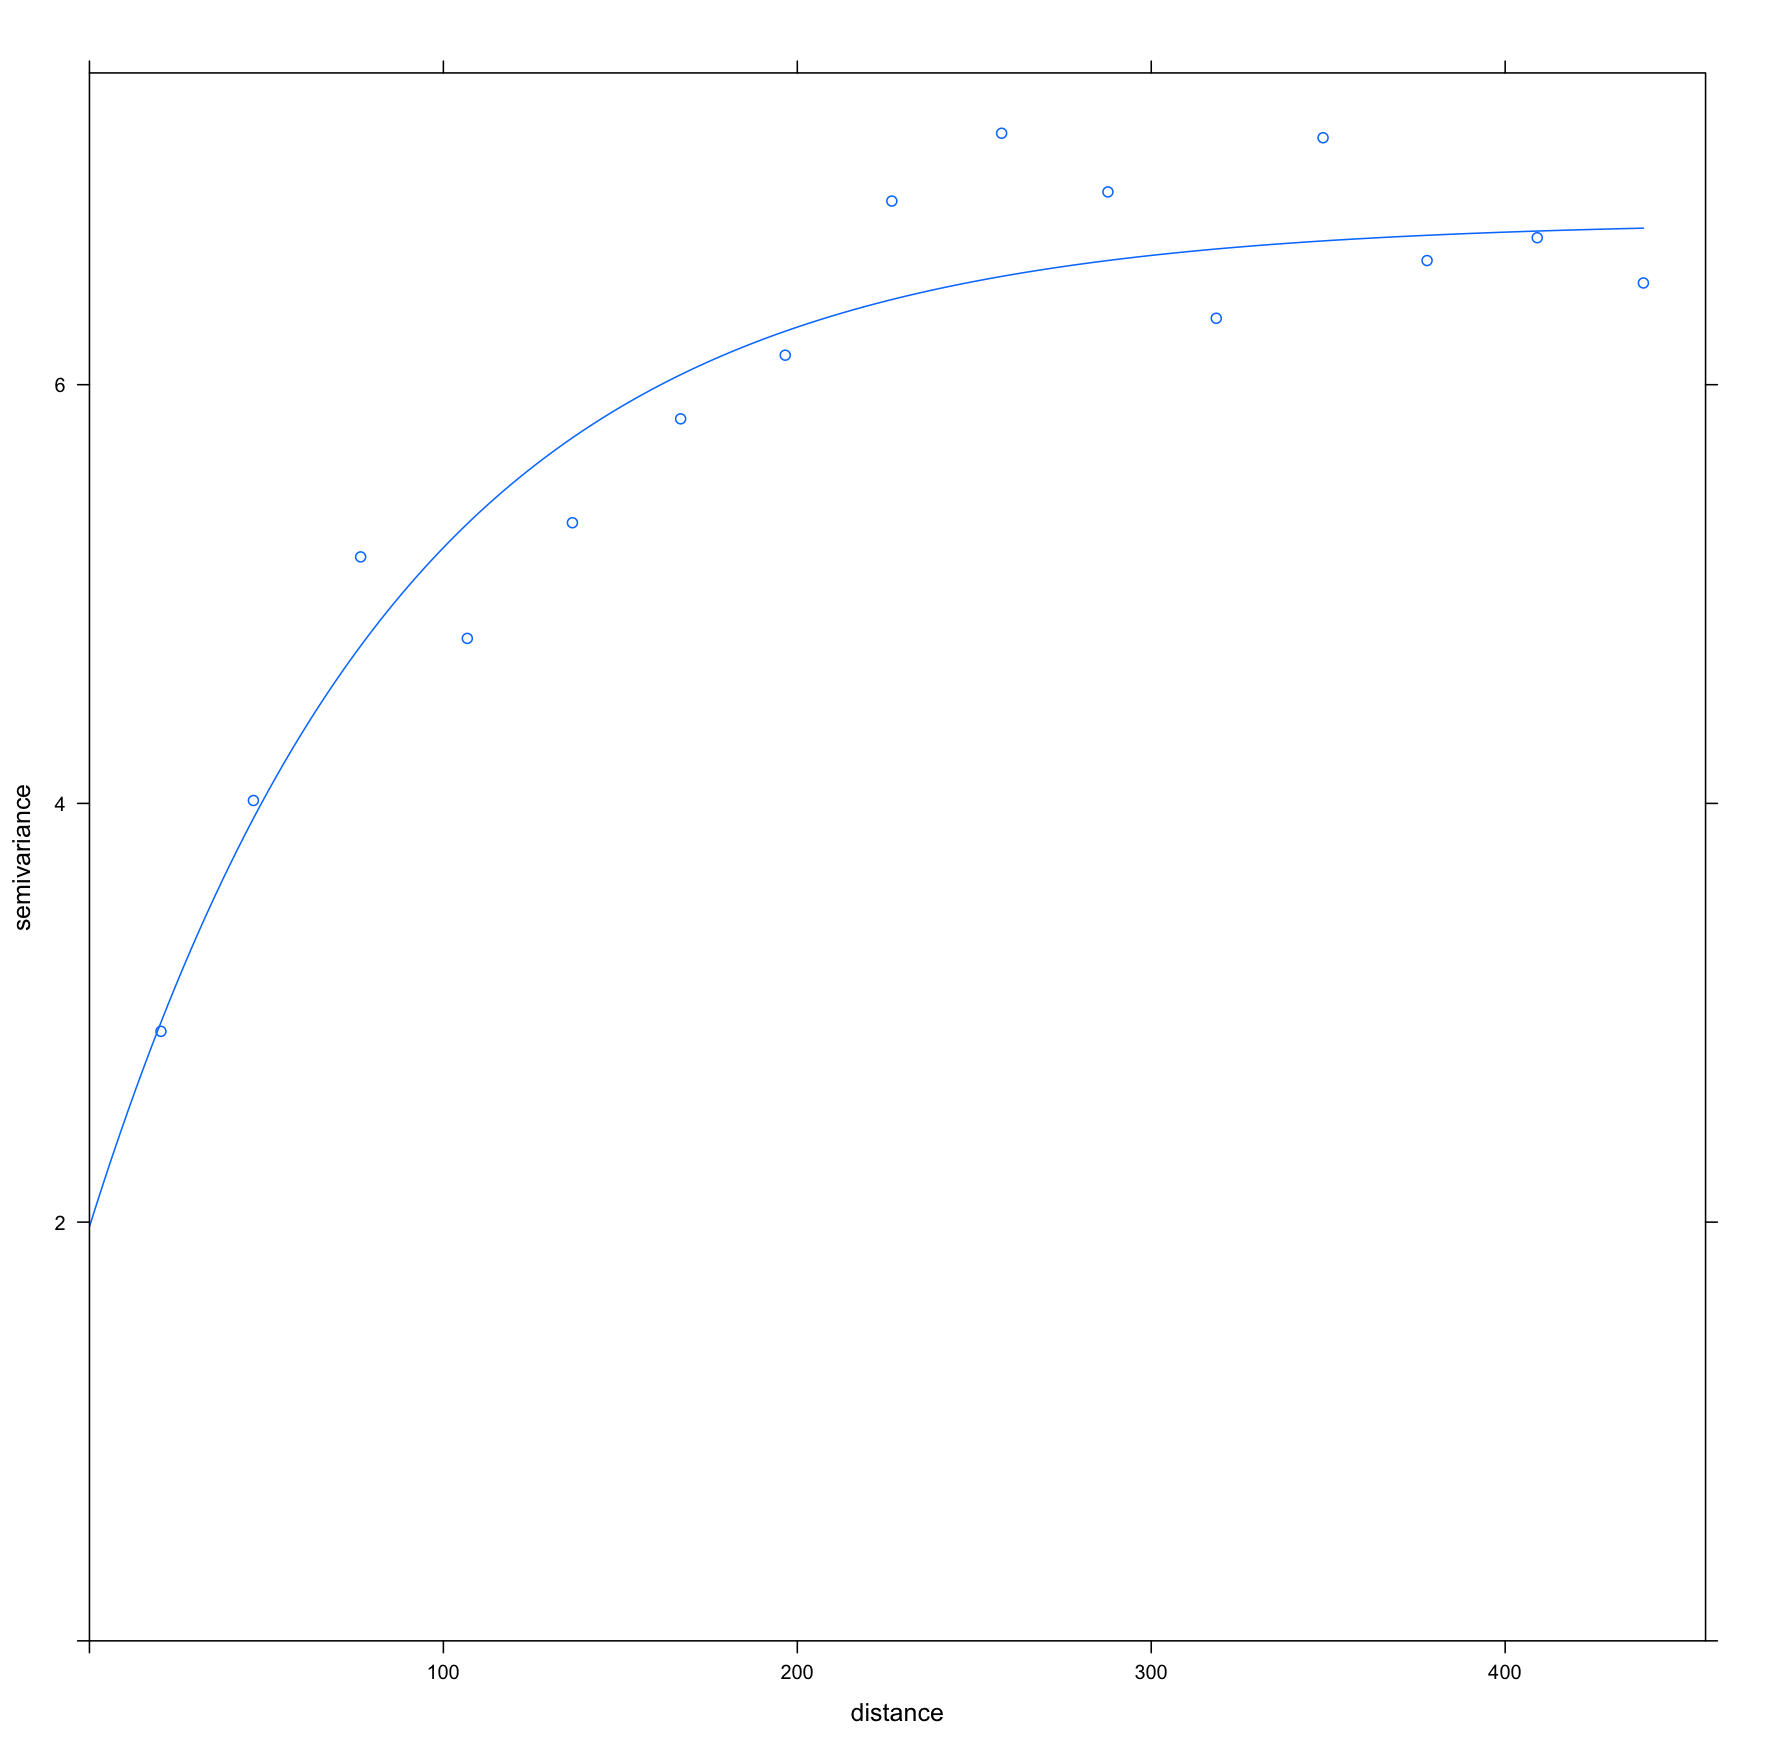
\includegraphics[width=\textwidth]{variogram.png}

\subsection*{(c)}
$\hat{\beta}_{gls} = (X'\Sigma X)^{-1}X'\Sigma^{-1}Y$, where $\hat{\Sigma}_{i,j} = C(s_{i}-s_{j})$ \\
$C(s_{i}, s_{j})$ is the exponential covariance function. \\

$C(s_{i}, s_{j})$ =
\left\{
    \begin{array}{ll}
        $\tau^2 + \sigma^2$  & \text{if } s_{i}-s_{j} = 0 \\
        $\sigma^2 exp(-\Vert s_{i}-s_{j} \Vert / \rho)$ & \text{else}
    \end{array}
\right.


\begin{lstlisting}
# Get distance matrix.
distance_matrix <- rdist(coordinates(CAtemp_with_coordinates))
dim(distance_matrix) # (200, 200)

# Create cov matrix.
exponential_covariance <- function(distance_matrix, tau_sqrd_hat, sigma_sqrd_hat, rho_hat){
  n = dim(distance_matrix)[1]
  matrix_with_no_nugget <- matrix(rep(0, n*n), ncol=n)
  print(dim(matrix_with_no_nugget))
  for (i in 1:n){
    for (j in 1:n){
      h = distance_matrix[i,j]
      matrix_with_no_nugget[i,j] <- sigma_sqrd_hat * exp(-h/rho_hat)
    }
  }
  matrix_with_nugget <- (sigma_sqrd_hat + tau_sqrd_hat) * diag(n)
  print(dim(matrix_with_nugget))
  return(matrix_with_no_nugget + matrix_with_nugget)
}
covariance_matrix_hat <- exponential_covariance(distance_matrix, tau_sqrd_hat, sigma_sqrd_hat, rho_hat)

# Invert covariance matrix and store.
inverse_covariance_matrix_hat <- solve(covariance_matrix_hat)

# Create X
X <- cbind(CAtemp$elevation, coordinates(CAtemp)); colnames(X) <- c('elevation', 'lon', 'lat')
y <- CAtemp$avgtemp

# Form beta_gls
(beta_gls <- solve(t(X) \%*\% inverse_covariance_matrix_hat \%*\% X) \%*\% t(X)\%*\% inverse_covariance_matrix_hat \%*\%y)
\end{lstlisting}
Betas for elevation, lon and lat is -0.006811685, -0.789559019, -0.961641363 respectively.


\subsection*{(d)}


 
\end{document}  